\icode{E-MD-CA-L3-261112-001}
木板和滑块摩擦系数 \(\mu_1 = 0.2\)，地面摩擦系数 \(\mu_2 = 0.1\)，木板质量为\(m_2 =\) \,\qty{0.5}{kg}，木块质量为\(m_1 =\) \,\qty{1}{kg}，物块以初速度 \(v_0 =\) \,\qty{4}{m/s}向右冲上静止的木板左端，木板足够长，求：
\begin{enumerate}
	\item \(m_1\) 和 \(m_2\) 相对位移；
	\item \(m_1\) 总运动时间。
\end{enumerate}

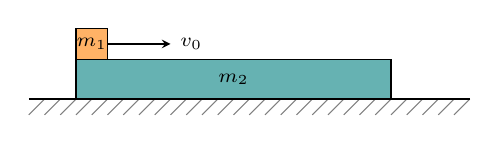
\begin{tikzpicture}[>=stealth,font=\scriptsize]
	\draw[fill=teal!60] (0,0) rectangle(4,.5)node[midway]{\(m_2\)};
	\draw[fill=orange!60] (0,.5) rectangle(.4,.9)node[midway]{\(m_1\)};
	\foreach \x in {-.6,-.4,...,5}
		\draw[gray] (\x,-.2)--++(.2,.2);
	\draw[thick] (-.6,0)--(5,0);
	\draw[->] (.4,.7)--++(.8,0)node[right]{\(v_0\)};
\end{tikzpicture}
\begin{answer}
	（1）\(\frac{8}{3}\)\qty{}{m}（2）\(\frac{8}{3}\)\qty{}{s}
\end{answer}